\section{Diseño interfaz de usuario inicial – wireframe}

{Dada la lógica en los casos de uso, se procede a estructurar la interfaz de usuario y la usabilidad de esta, teniendo en cuenta a los usuarios objetivo, quienes son personas de baja escolaridad y con un bajo dominio de los medios tecnológicos, por tal motivo, la interfaz debe ser sencilla, con pocos botones e intuitiva, nos apoyamos en la guía visual “wireframe” que nos posibilito la creación de un esqueleto o estructura inicial del sitio WEB, dando como resultado lo siguiente:

\begin{figure}[H]
	\centering
	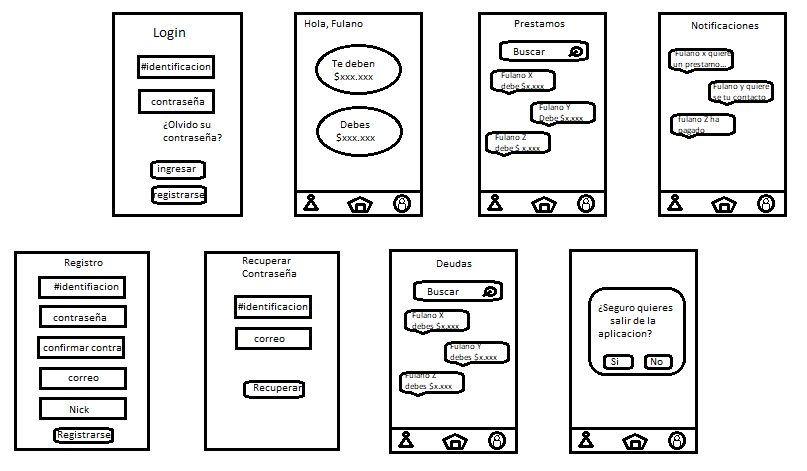
\includegraphics[width=1\linewidth]{development/wireframe.png}
	\caption{Wireframe}
\end{figure}
\begin{center}
	\textbf{Fuente:} Propia.
\end{center}
}